\documentclass[xcolor={rgb}]{beamer}
\usepackage[labelformat=empty]{caption}
\usepackage[outputdir=out]{minted}

\newcommand{\pitem}{\pause\item}
\usetheme{metropolis}

\author{Alireza Arzehgar}
\title{Leaderless Replication}
\date{\today}

\begin{document}
	\begin{frame}[plain]
		\titlepage
	\end{frame}

	\begin{frame}{Scaling to Higher Load}
		\begin{itemize}
			\pitem \textit{Vertical Scaling}
			\begin{itemize}
				\pitem Shared-Memory Architectire
				\pitem Shared-Disk Architectire
			\end{itemize}
			\pitem \textit{Horizontal Scaling}
			\begin{itemize}
				\pitem Shared-Nothing Architectire
			\end{itemize}
		\end{itemize}
	\end{frame}

	\begin{frame}{Replication}
		\begin{itemize}
			\pitem What is Replication?
			\pitem Leaders and Followers
			\pitem Reasons why you might want to replicate data
			\begin{itemize}
				\pitem Latency
				\pitem Fault tolerance/high availability
				\pitem Scalability
			\end{itemize}
		\end{itemize}
	\end{frame}

	\begin{frame}{Algorithms for replicating changes between nodes}
		\begin{itemize}
			\pitem Single-leader replication
			\pitem Multi-leader replication
			\pitem Leaderless replication
		\end{itemize}
	\end{frame}

	\begin{frame}{Single-Leader Replication}
		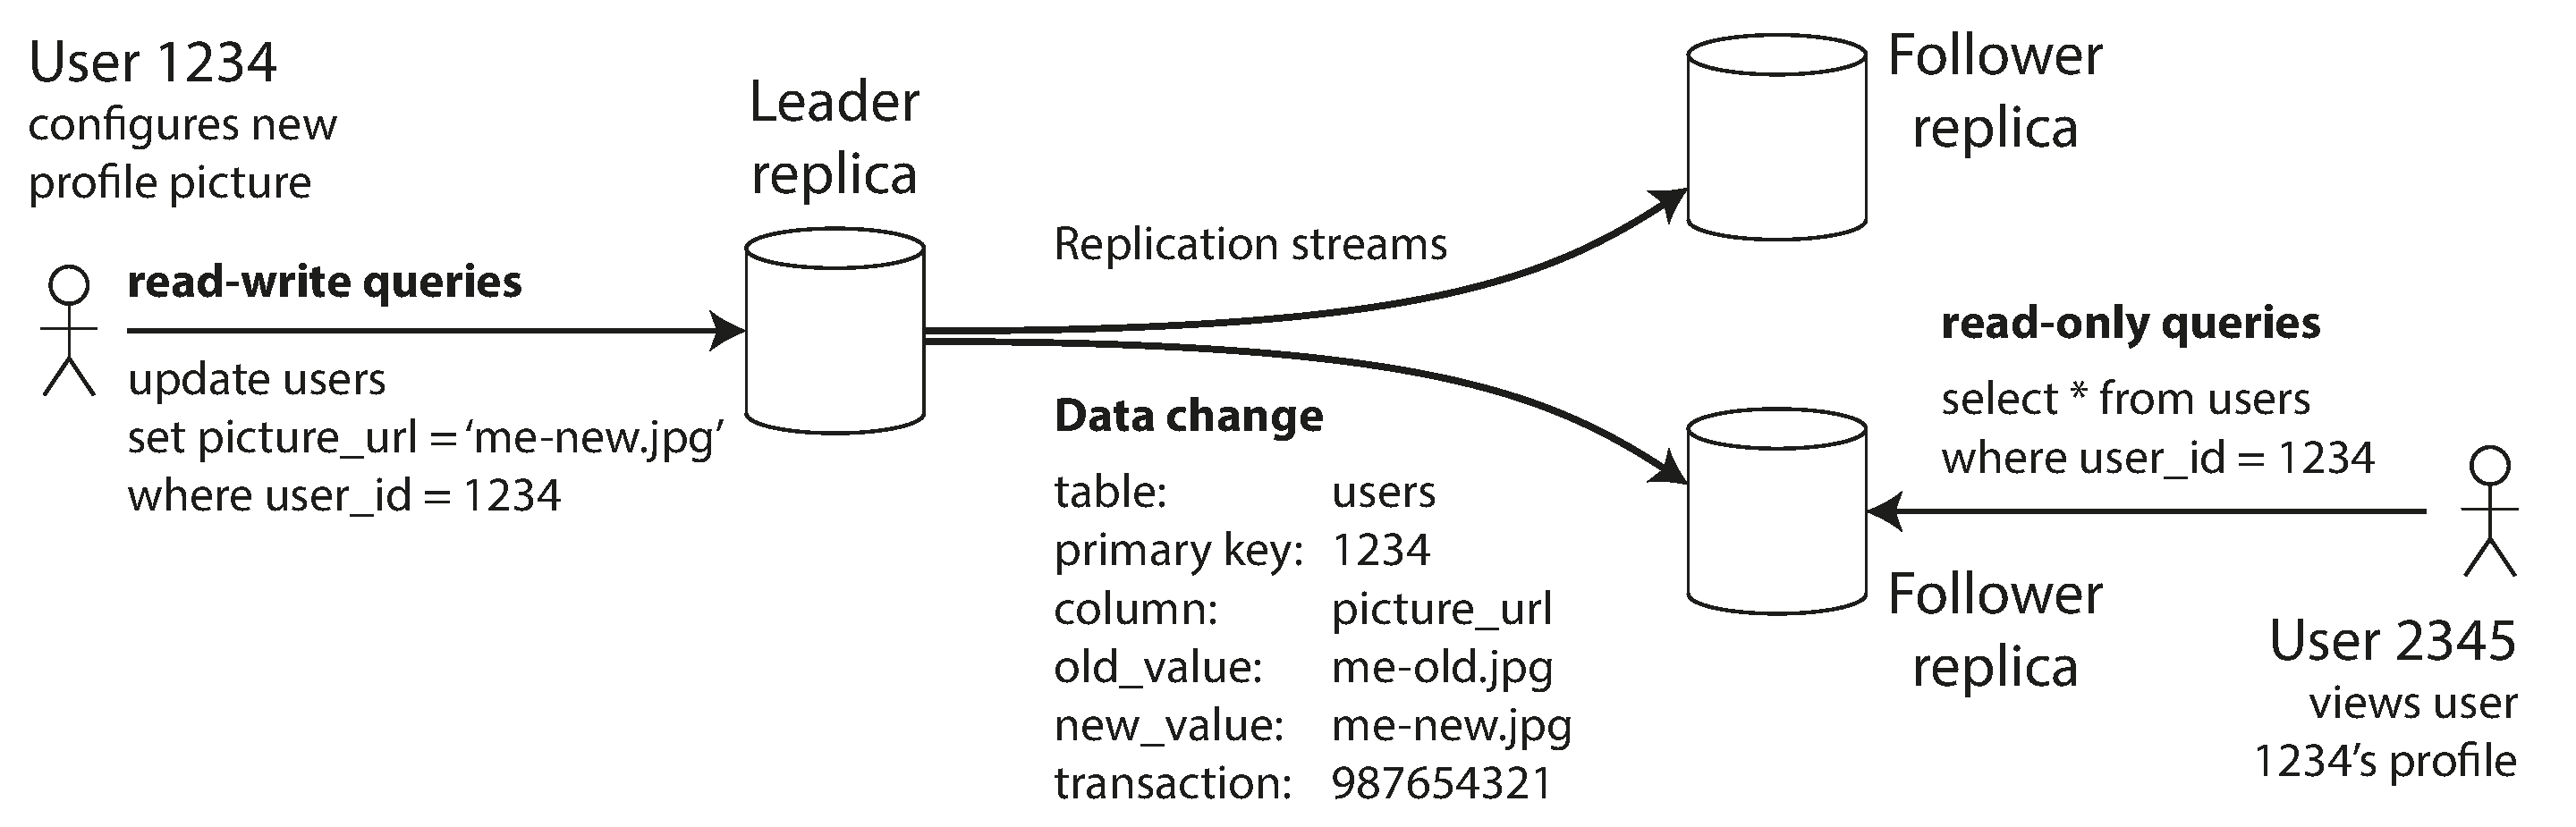
\includegraphics[width=\textwidth]{assets/single-leader-replication.png}
		\textbf{Databases with single-leader replication support}:
		\begin{itemize}
			\item \textbf{SQL}: PostgreSQL, MySQL, Oracle Data Guard
			\item \textbf{NoSQL}: MongoDB, RethinkDB, CouchDB, Redis, Neo4j
			\item \textbf{Others}: Kafka, RabbitMQ, NATS, DRBD
		\end{itemize}
	\end{frame}

	\begin{frame}{Multi-Leader Replication}
		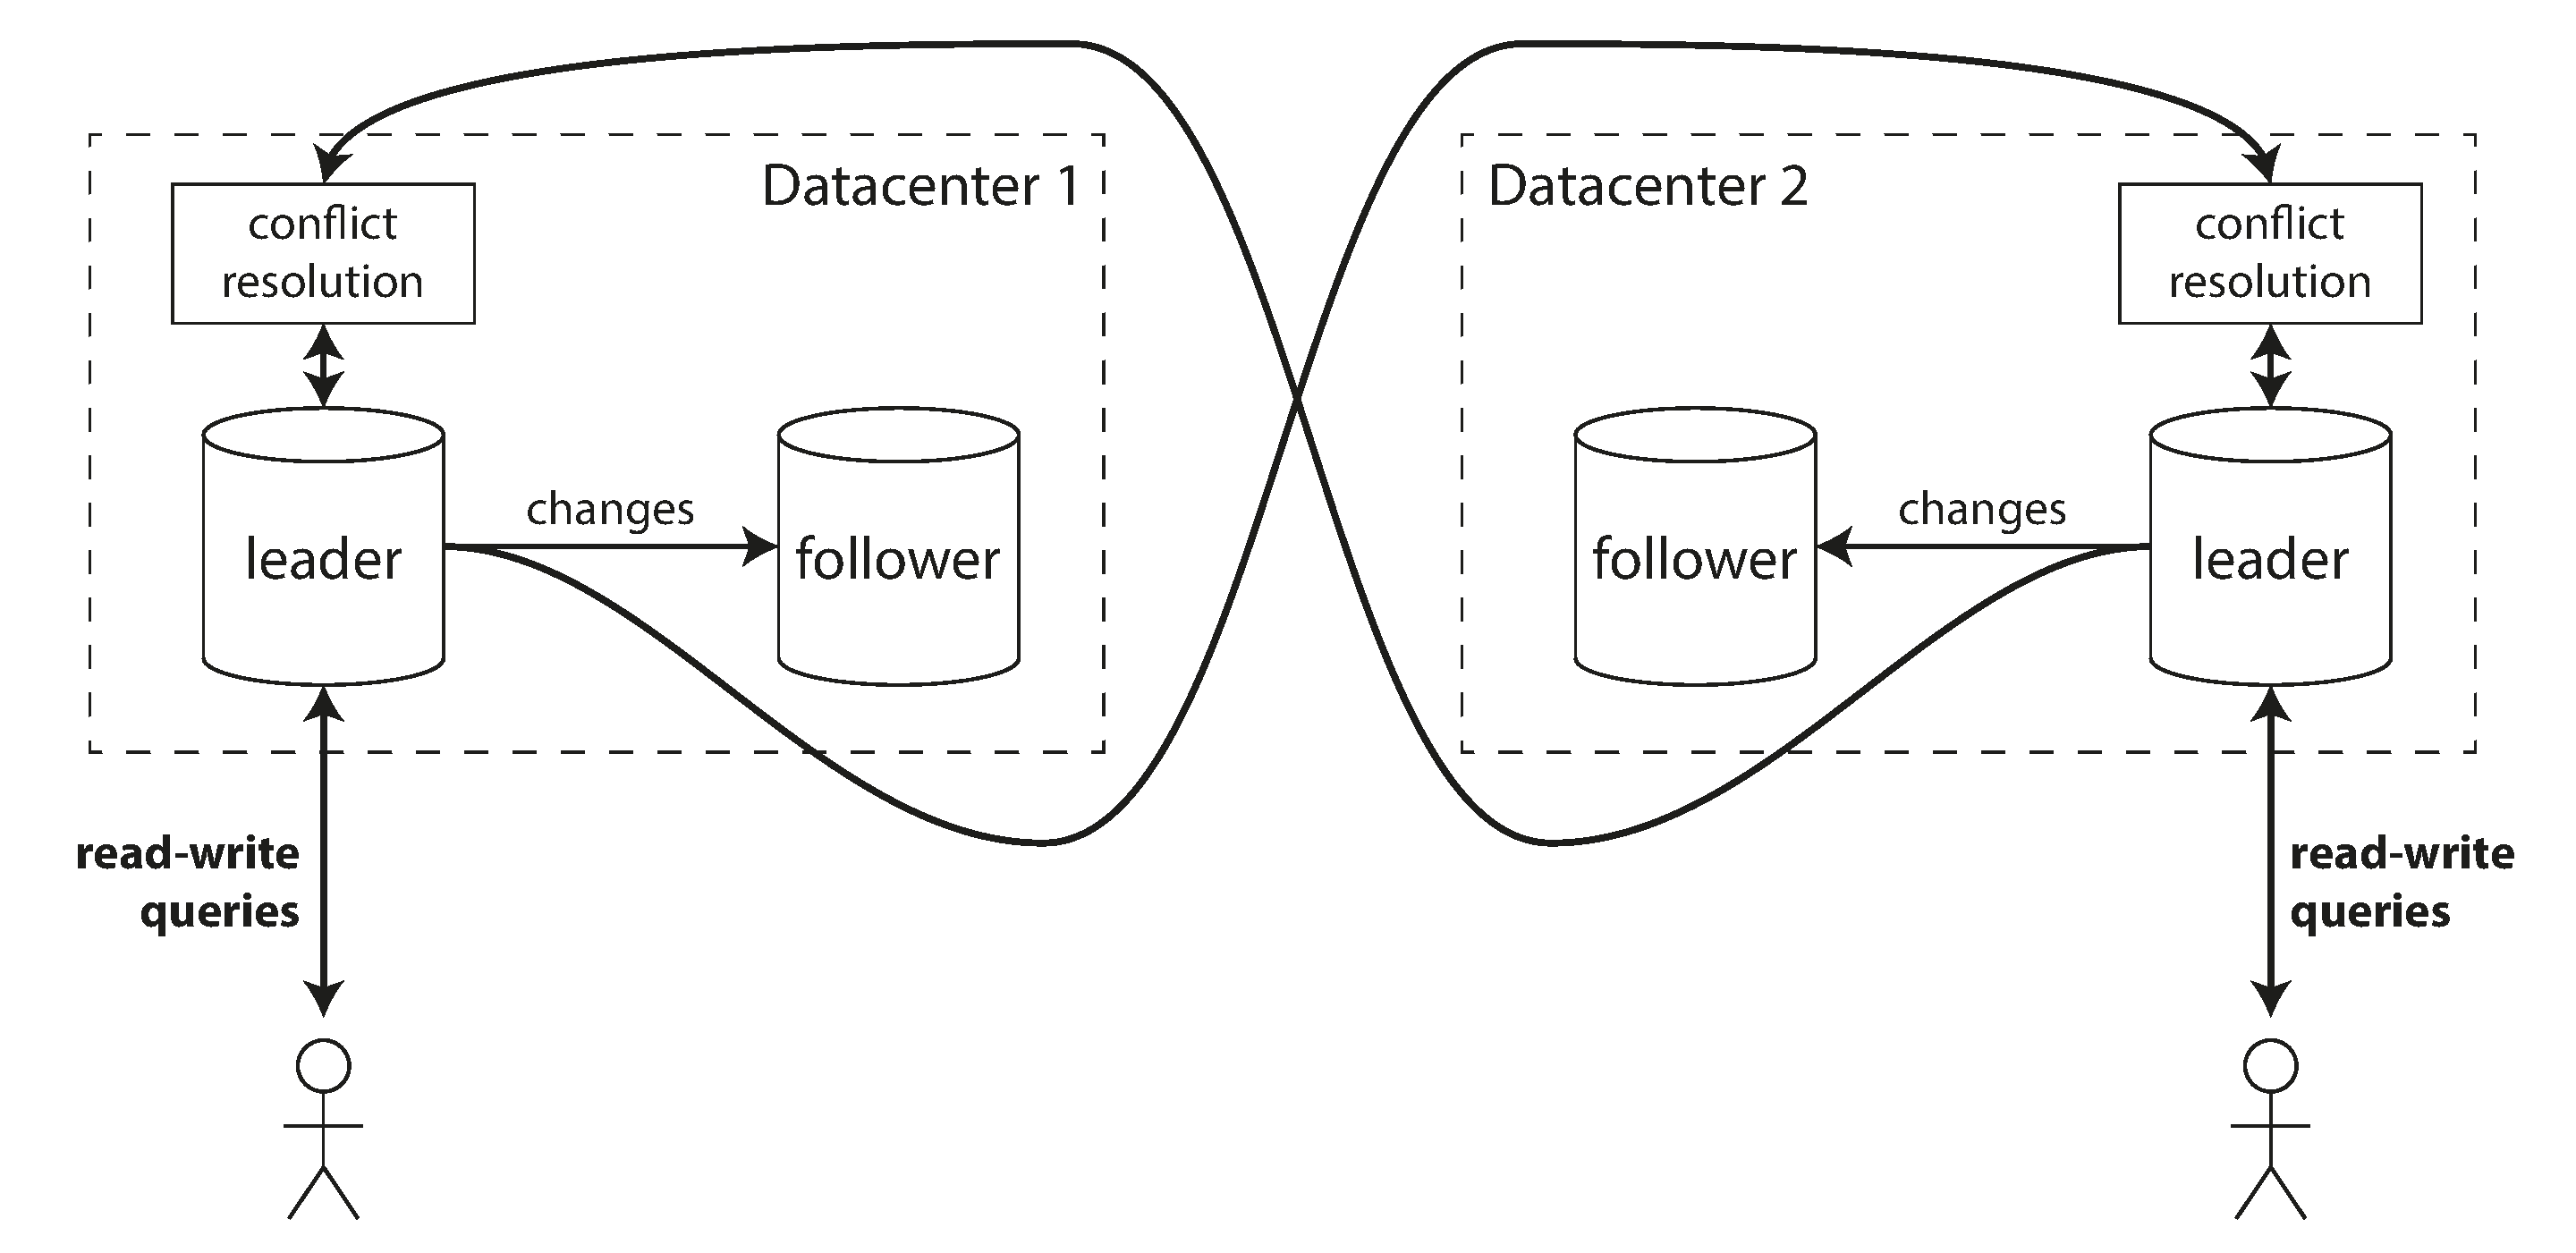
\includegraphics[width=\textwidth]{assets/multi-leader-replication.png}
		\textbf{Compare with single-leader replication}:
		\begin{itemize}
			\pitem Performance
			\pitem Tolerance of datacenter outages
			\pitem Tolerance of network problems
		\end{itemize}
	\end{frame}

	\begin{frame}{Leaderless Replication}
		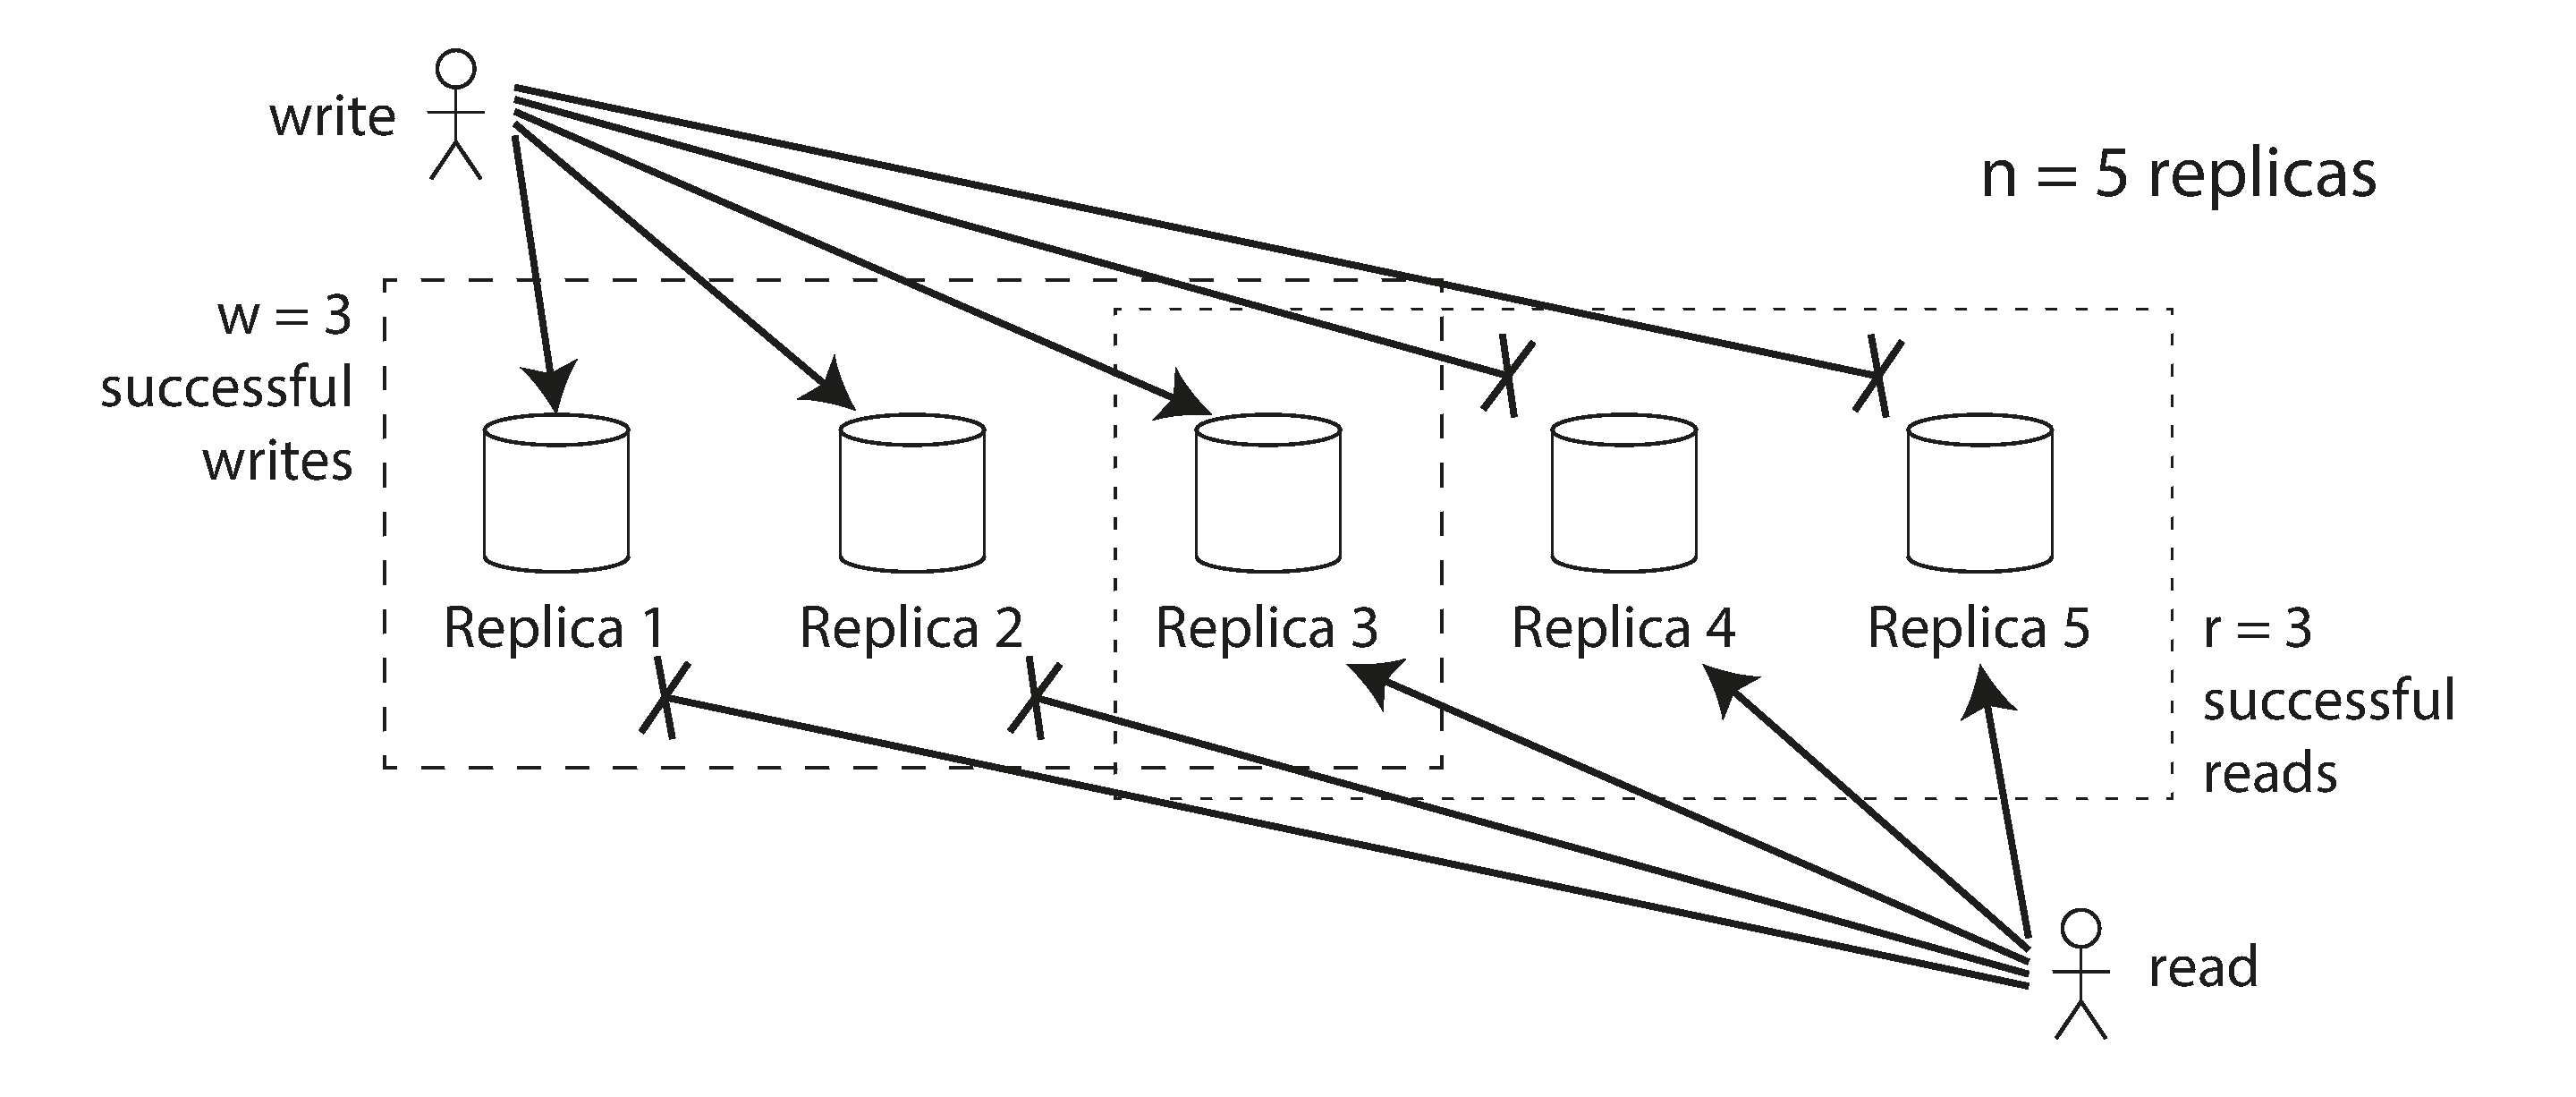
\includegraphics[width=0.9\textwidth]{assets/quorum.png}
		\begin{itemize}
			\pitem \textbf{Mechanism}: Read \& write on all nodes
			\pitem \textbf{Databases}: Amazon DynamoDB, Cassandra, ScyllaDB, Riak
		\end{itemize}
	\end{frame}

	\begin{frame}{Quorum}
		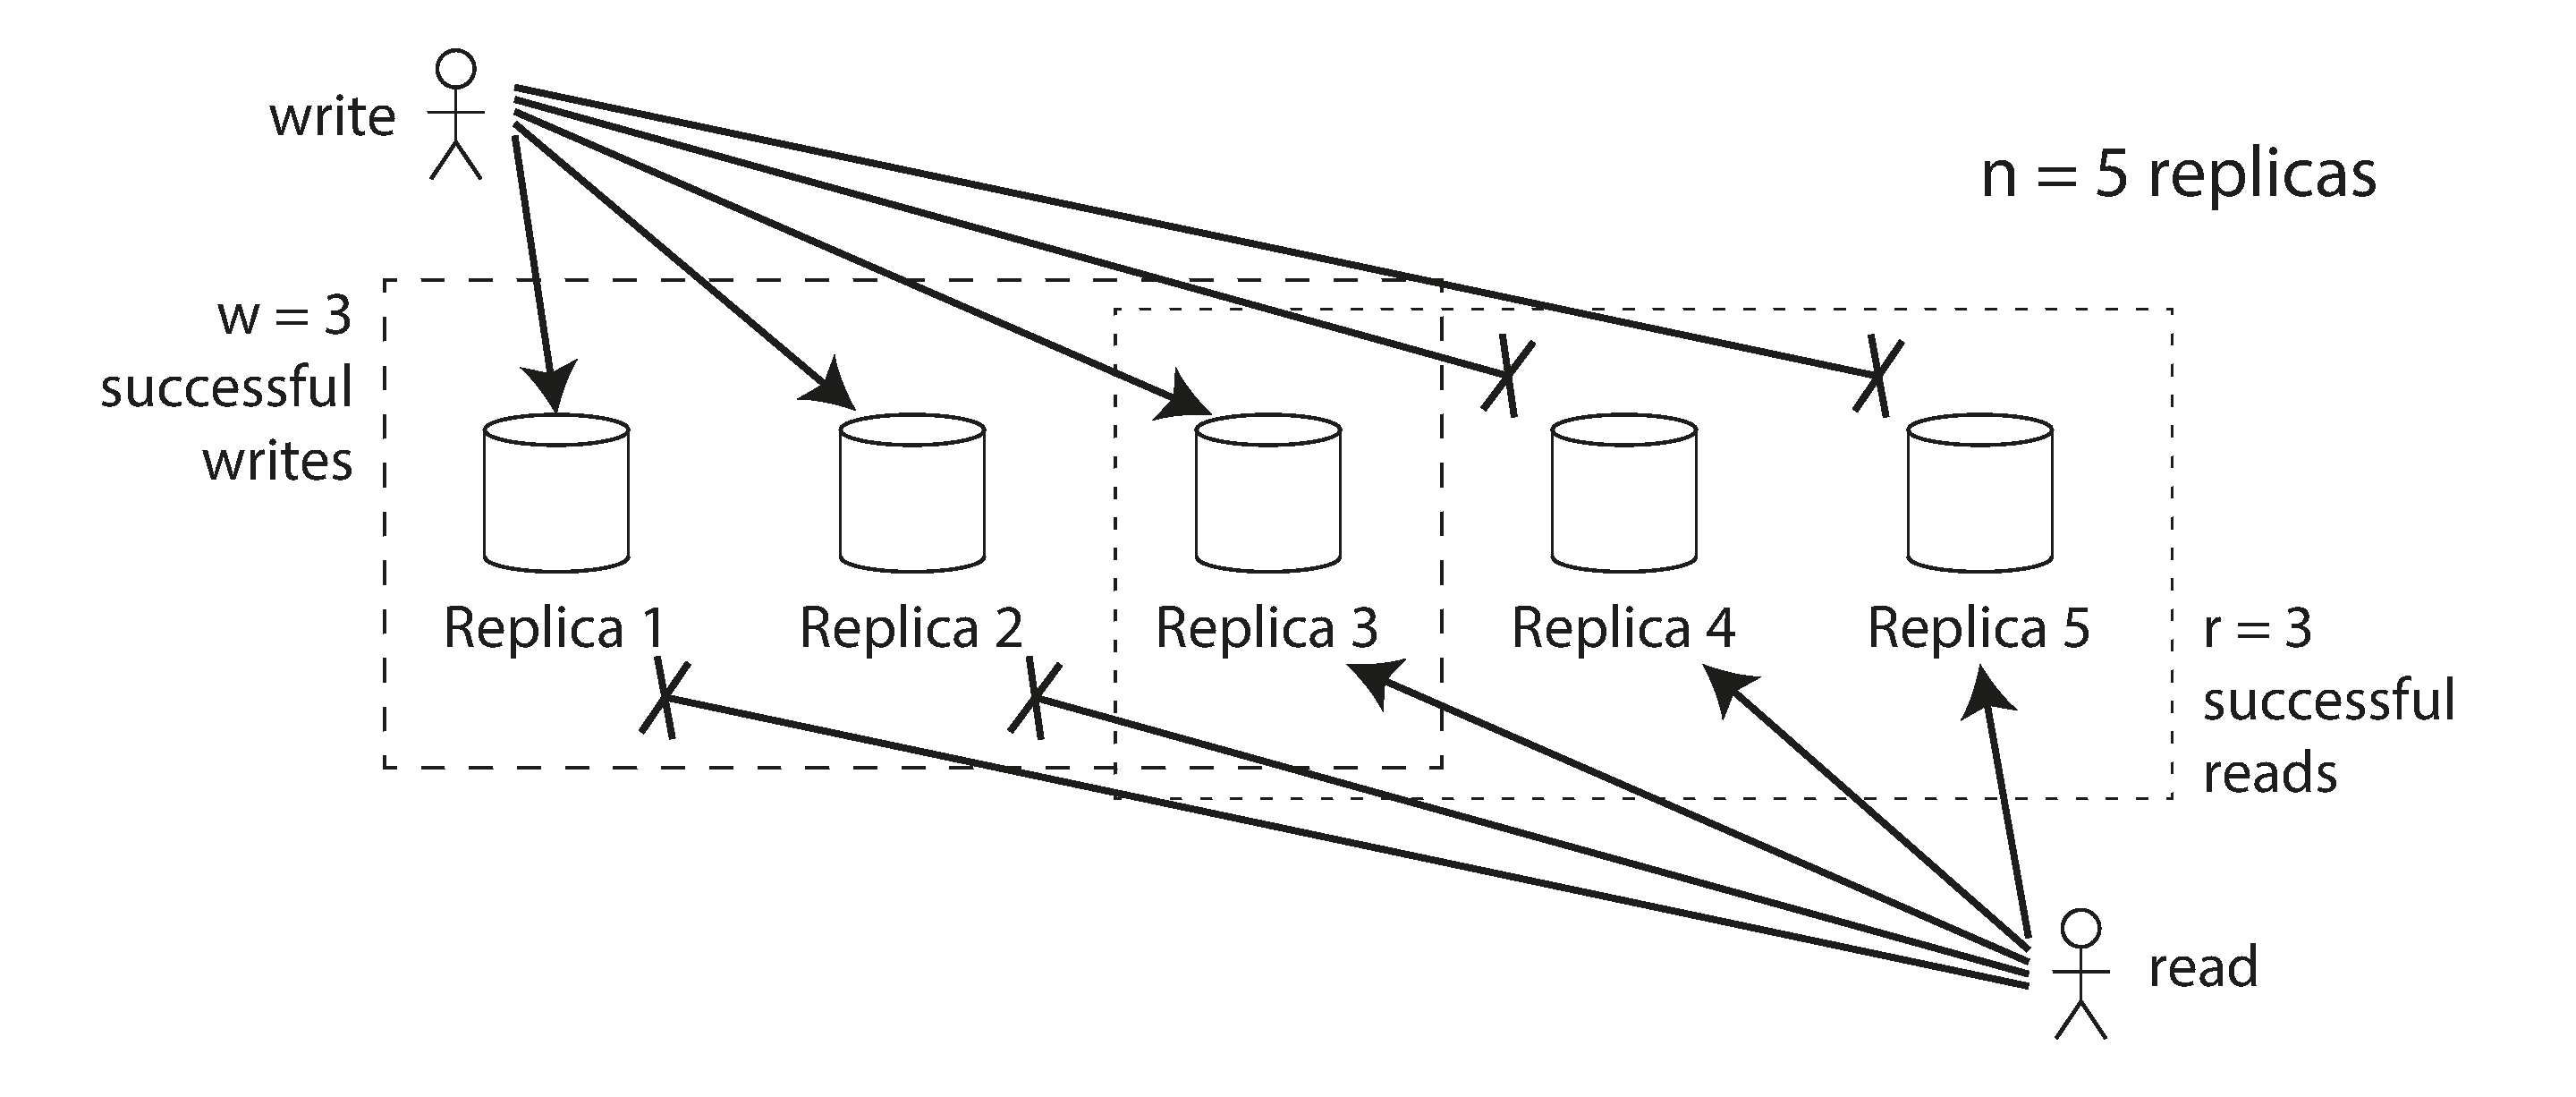
\includegraphics[width=0.9\textwidth]{assets/quorum.png}
		\begin{itemize}
			\pitem \textbf{Quorum Factors}
			\begin{itemize}
				\pitem Number of nodes: $n$
				\pitem Sync writes: $w$
				\pitem Sync reads: $r$
			\end{itemize}
			\pitem \textbf{Condition}: $w + r > n$
			\pitem \textbf{Recommendation}: $w = r = (n + 1) / 2$
		\end{itemize}
	\end{frame}

	\begin{frame}{How to handle inconsistencies}
		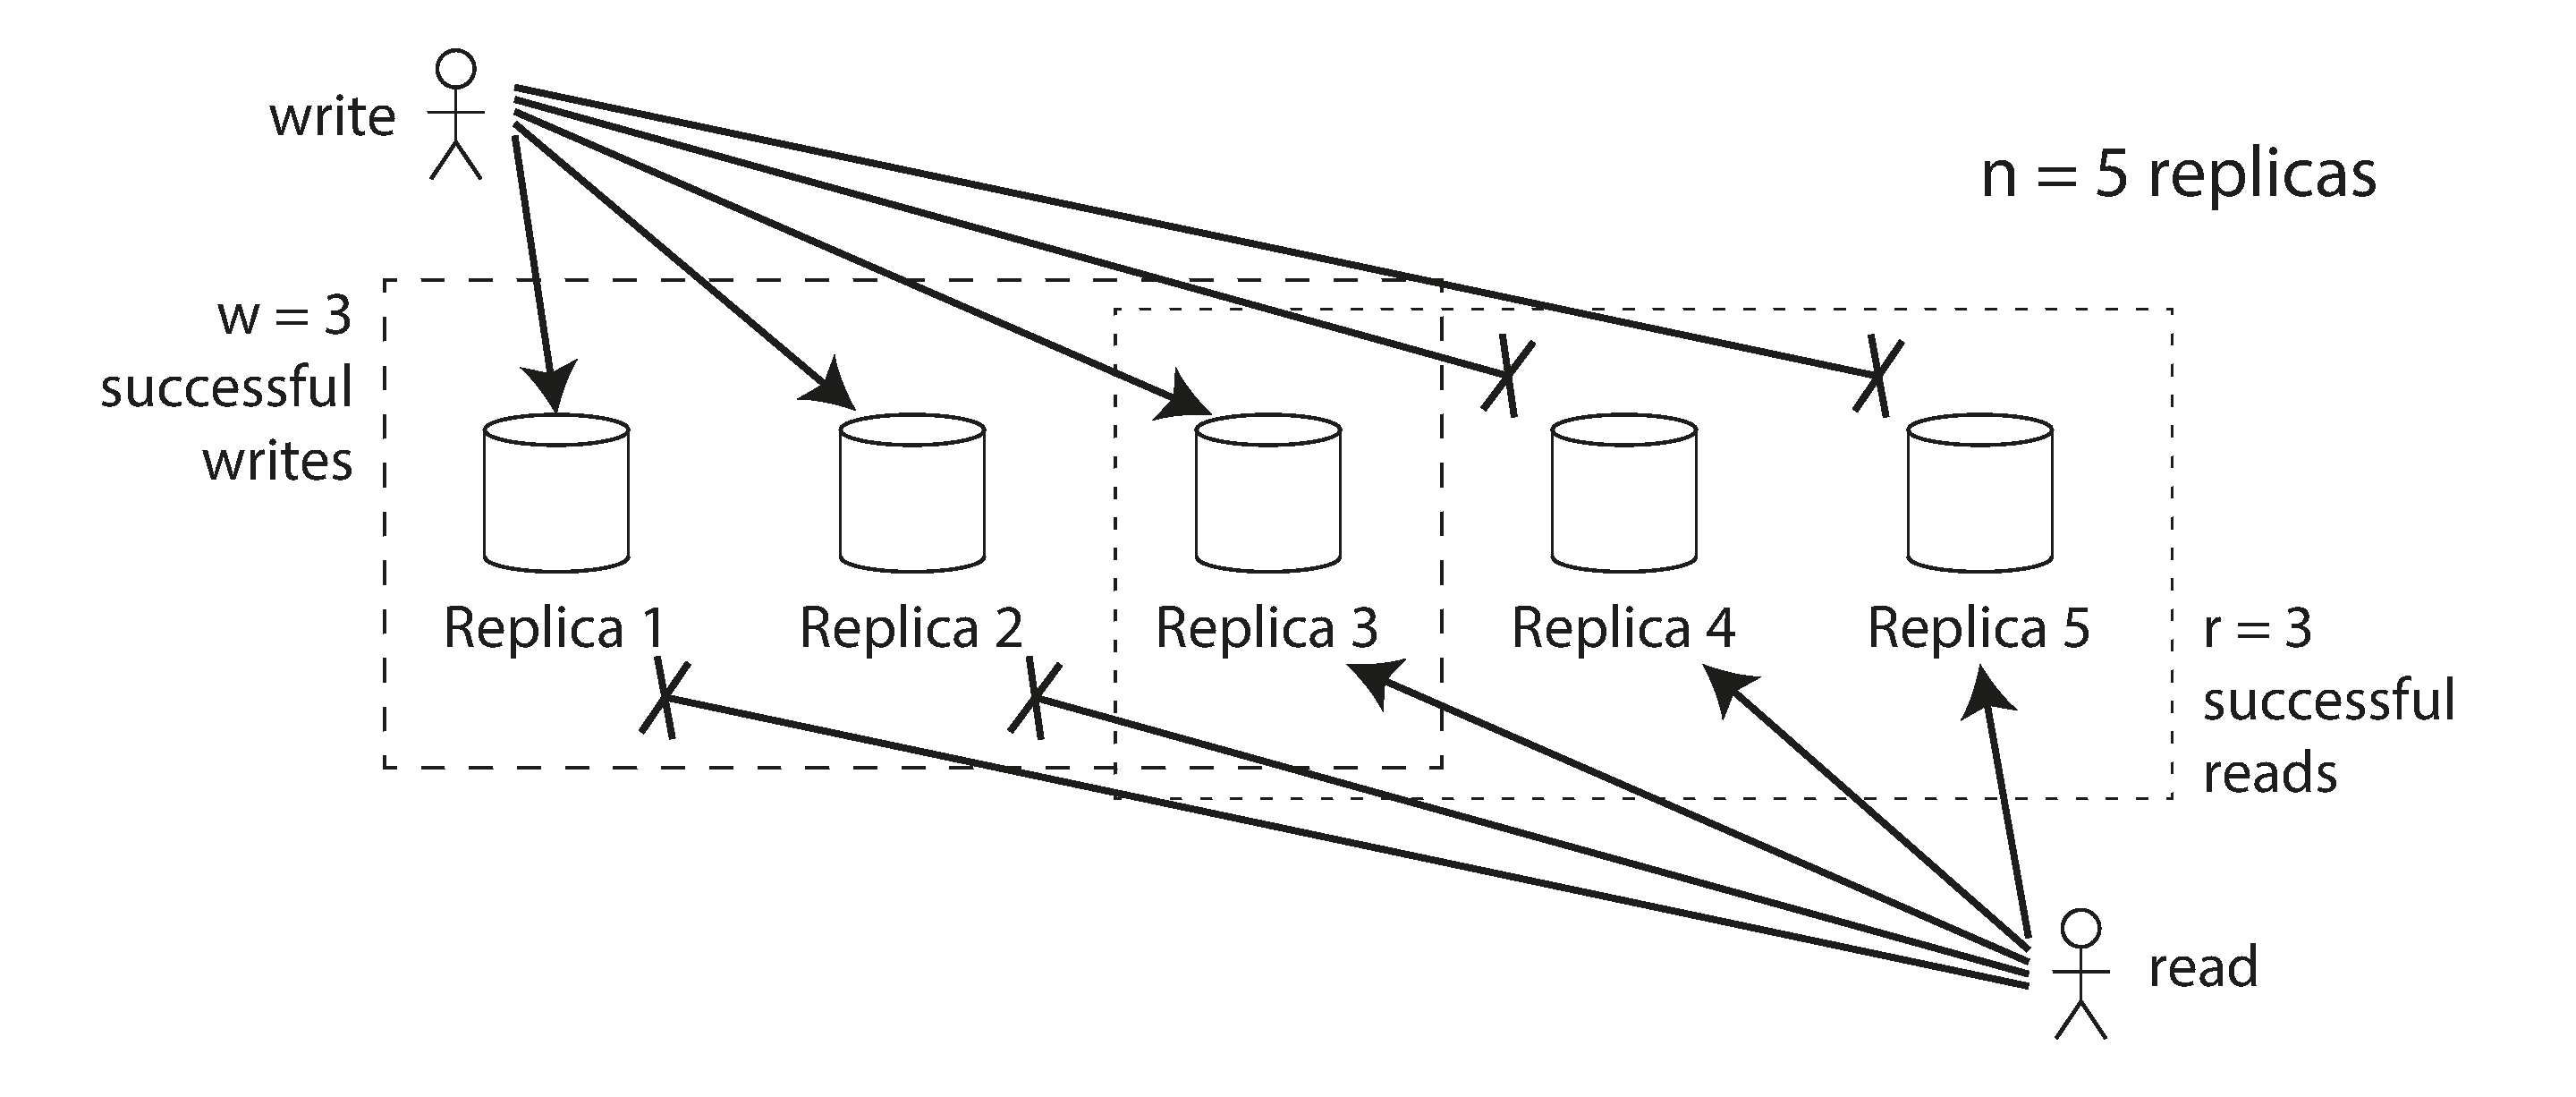
\includegraphics[width=\textwidth]{assets/quorum.png}
		\begin{itemize}
			\pitem Read repair
			\pitem Anti-entropy process
		\end{itemize}
	\end{frame}

	\begin{frame}{More High Availability}
		\begin{itemize}
			\pitem Sloppy Quorum
			\pitem Hinted Handoff
			\pitem $w + r > n$ can be inconsistent
			\pitem Availablity \& Consistency Trade-Off
		\end{itemize}
	\end{frame}

	\begin{frame}{Cassandra \& ScyllaDB Consistency Levels}
		\begin{itemize}
			\pitem ALL: w = n, r = n
			\pitem ONE: w = 1, r = 1
			\pitem QUORUM: w = r = (n//2) + 1
			\pitem ANY (Hinted Handoff): w = 1, r = 1
			\pitem LOCAL\_ONE
			\pitem LOCAL\_QUORUM
			\pitem EACH\_QUORUM
		\end{itemize}
	\end{frame}

	\begin{frame}[plain,c]
		\begin{center}
		\Huge Near-World Example
		\end{center}
	\end{frame}

	\begin{frame}{About Our Mission}
		\begin{itemize}
			\pitem ScyllaDB
			\pitem Docker Compose
			\pitem Golang
			\pitem Tmux
		\end{itemize}
	\end{frame}

	\begin{frame}[fragile]{ScyllaDB Cluster}
		\begin{minted}[fontsize=\tiny]{yaml}
version: "3.3"
services:
  scylla1:
    container_name: scylla1
    image: docker.arvancloud.ir/scylladb/scylla:latest
    ports:
      - 9001:9042
  scylla2:
    container_name: scylla2
    image: docker.arvancloud.ir/scylladb/scylla:latest
    ports:
      - 9002:9042
    command: --seeds=scylla1
  scylla3:
    container_name: scylla3
    image: docker.arvancloud.ir/scylladb/scylla:latest
    ports:
      - 9003:9042
    command: --seeds=scylla1
		\end{minted}

		\pause
		\begin{minted}[fontsize=\tiny]{shell}
$ docker-compose up -d
$ docker exec -it scylla1 nodetool status
Datacenter: datacenter1
=======================
-- Address    Load      Tokens Owns Host ID                              Rack 
UN 172.23.0.2 797.73 KB 256    ?    e43a9696-3de7-45e6-b224-0a435d734ee3 rack1
UN 172.23.0.3 591.56 KB 256    ?    8ac23529-ee87-4537-bd97-de7140a51649 rack1
UN 172.23.0.4 779.90 KB 256    ?    e6088a14-5e8e-44d8-a902-c56f1e81d316 rack1
		\end{minted}
	\end{frame}

	\begin{frame}[fragile]{ScyllaDB Client}
		\begin{minted}[fontsize=\scriptsize]{go}
cluster := gocql.NewCluster(
	"localhost:9001", "localhost:9002", "localhost:9003"
)
cluster.Consistency = gocql.Quorum
session, _ := cluster.CreateSession()

session.Query(
  `CREATE KEYSPACE IF NOT EXISTS test
  WITH REPLICATION = {'class': 'SimpleStrategy', 'replication_factor': '3'}`,
).Exec()
session.Query(`CREATE TABLE IF NOT EXISTS test.users (
  id UUID PRIMARY KEY, username text, email text
)`).Exec()

for range 100000 {
  uuid := fmt.Sprint(gocql.UUIDFromTime(time.Now()))
  q := `INSERT INTO test.users (id, username, email) VALUES (?, ?, ?)`
  session.Query(q, uuid, "username", "mock@email.com").Exec()
}
		\end{minted}
	\end{frame}

	\begin{frame}{Check replicas}
		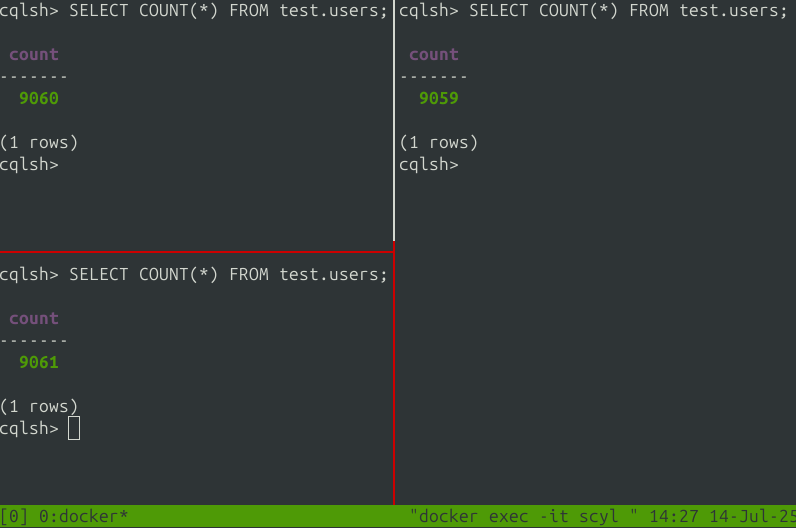
\includegraphics[width=\textwidth]{assets/scylladb_inconsistency.png}
	\end{frame}
\end{document}
